\documentclass{beamer}
\usetheme{PaloAlto}

\title{Implementacion de la Factorizacion Cholesky con openMP}

% A subtitle is optional and this may be deleted
\subtitle{Aplicacion}

\author{Alejandro Nivon\inst{1} \and Uriel Miranda\inst{1} \and Hector Corro\inst{1}}
% - Give the names in the same order as the appear in the paper.
% - Use the \inst{?} command only if the authors have different
%   affiliation.

\institute[Universities of Somewhere and Elsewhere] % (optional, but mostly needed)
{
  \inst{1}%
  Maestria en Ciencia de Datos\\
  ITAM
}  
\date{MNO - 2018, Mayo 2018}
% - Either use conference name or its abbreviation.
% - Not really informative to the audience, more for people (including
%   yourself) who are reading the slides online

\subject{Theoretical Computer Science}
% This is only inserted into the PDF information catalog. Can be left
% out. 

% If you have a file called "university-logo-filename.xxx", where xxx
% is a graphic format that can be processed by latex or pdflatex,
% resp., then you can add a logo as follows:

% \pgfdeclareimage[height=0.5cm]{university-logo}{university-logo-filename}
% \logo{\pgfuseimage{university-logo}}

% Delete this, if you do not want the table of contents to pop up at
% the beginning of each subsection:
\AtBeginSubsection[]
{
  \begin{frame}<beamer>{Contenido}
    \tableofcontents[currentsection,currentsubsection]
  \end{frame}
}

% Let's get started
\begin{document}

\begin{frame}
  \titlepage 
\end{frame}

\begin{frame}{Contenido}
  \tableofcontents
  % You might wish to add the option [pausesections]
\end{frame}

% Section and subsections will appear in the presentation overview
% and table of contents.
\section{Primera Parte}

\subsection{Objetivo}

\begin{frame}{Introduccion}{Motivacion}
  \begin{itemize}
  \item {
    \textbf{Objetivo.}
  }
  \begin{itemize}
  \item {
    Aprovechar las oportunidades creadas o generadas por las tecnologias actuales para la paralelizacion de rutinas del calculo numerico.
  	}
  \end{itemize}  	
  \end{itemize}
\end{frame}

\subsection{Factorizacion Cholesky}

% You can reveal the parts of a slide one at a time
% with the \pause command:
\begin{frame}{Factorizacion Cholesky}
  \begin{itemize}
  \item {
    Para matrices positivas definidas. 
  }
  \item {   
    Las matrices positivas definidas pueden ser expresadas de la forma $A = X^TX$ para una matriz $X$ no singular.
  }
  \item{
  	La factorizacion Cholesky es una forma particular de factorizar $X$, en la que $X$ es la matriz triangular superior con elementos positivos en su diagonal; generalmente es escrito como: \(A = R^TR\) o $A = LL^T$ de una matriz definida \(A\), en la que \(R\) es una matriz triangular superior con elementos positivos en su diagonal es una herramienta fundamental para su calculo matricial.
  } 
    \end{itemize}
\end{frame}

\begin{frame}{Factorizacion Cholesky}
\begin{block}{\textbf{Lemma 1.1}}
Sea \(A\) positiva semi-definida de rango \(r\)
\end{block}
\begin{enumerate}
\item Existe al menos una matriz triangular superior \(R\) con elementos no negativos en su diagonal tal que \(A = R^TR\).
\end{enumerate} 

\begin{enumerate}
\item Hay una permutacion $\prod$ tal que $\prod^TA\prod$ tiene una unica factorizacion cholesky que toma la forma: 
\end{enumerate}

\begin{equation}
\prod^TA\prod = R^TR ,
\end{equation}

\[
R = 
 \begin{pmatrix}
  r_{1,1} & r_{1,2} \\
  0 & 0
 \end{pmatrix}
\]
\end{frame}

\begin{frame}{Factorizacion Cholesky}
\begin{itemize}
\item \textbf{Aplicaciones}
	\begin{itemize}
		\item La descomposicion de Cholesky se usa principalmente para hallar la solucion numerica de ecuaciones lineales $Ax = b$. Si $a$ es simetrica y positiva definida, entonces se puede solucionar $Ax = b$ calculando primero la descomposicion de Cholesky $A = LL^T$, luego resolviendo $Ly = b$ para $y$, y finalmente resolviendo $L^Tx = y$ para $x$.
	\end{itemize}
\item Ejemplos:
	\begin{itemize}
		\item Minimos cuadrados lineales
		\item Simulacion de Monte Carlo
		\item Filtro de Kalman
	\end{itemize}	 
\end{itemize}
\end{frame}

\section{Implementacion}

\subsection{Algoritmo}

\begin{frame}{Algoritmo}{Calculo}
La Factorizacion Cholesky puede ser calculada por una forma de eliminacion gaussiana que toma ventaja de la simetria y definicion. Iterando $(i,j)$, elementos en la ecuacion $A = R^TR$ como se ve a continuacion:

\begin{equation}
\j = i \qquad a_{ii} = {\displaystyle\sum_{k=1}^{i}{r^2_{ki}}}
\end{equation}

\begin{equation}
\j>i \qquad a_{ij} = {\displaystyle\sum_{k=1}^{i}{r_{ki}}{r_{kj}}}
\end{equation}
\end{frame}

\begin{frame}{Algoritmo}
\begin{itemize}
\item \textbf{Algoritmo} las ecuaciones anteriores pueden ser resueltas para producir $R$ columnas a la vez de la siguiente manera:
\end{itemize}
\begin{figure}[h]
    \centering
    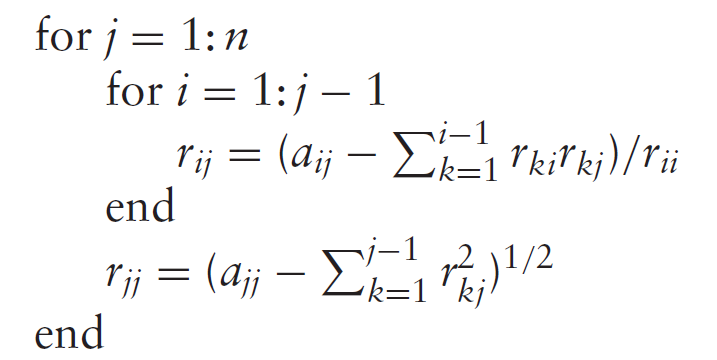
\includegraphics[width=0.5\textwidth]{for_cycle}
    \label{fig:mesh1}
\end{figure}
\end{frame}

\begin{frame}{Algoritmo}
Despues de investigar diferentes aproximaciones y formas de desarrollar la factorizacion de Cholesky, asi como su implementacion, se decidio paralelizar con base en el calculo de filas. Para esto lo mas importante a considerar es el orden en que se realizan los cálculos
\begin{itemize}
\item Elementos en la diagonal
\begin{equation}
\L_{ij}=\sqrt{A_{ij} - {\displaystyle\sum_{k=1}^{j-1} L^2_{jk}}} 
\end{equation}
\item Elementos bajo la diagonal
\begin{equation}
\L_{ij} = \frac{1}{L_{jj}} \big( A_{ij} - {\displaystyle\sum_{k=1}^{j-1} L_{ik}L_{jk}}\big)
\end{equation}
\end{itemize}
\end{frame}

\begin{frame}
Iniciando por el elemento $l_{11}$:

Aplicando la fórmula para elementos en la diagonal, tenemos:

\begin{equation}
\l_{11} = \sqrt{a_{11}}
\end{equation}

Para calcular el elemento $l_{21}$:

\begin{equation}
\l_{21} = \sqrt{a_{21}}
\end{equation}

Por lo cual para cada elemento de la columna j=1 no requiere dependencia de ningún otro elemento, por lo cual se puede realizar en paralelo.

\end{frame}

\begin{frame}
Siguiendo con esa línea para calcular el elemento $l_{32}$

\begin{equation}
\l_{32} = \frac{1}{l_{33}} \big( a_{32} - {l_{31}l_{21}}\big)
\end{equation}

Comparamos con el cálculo del elemento  $l_{42}$:

\begin{equation}
\l_{42} = \frac{1}{l_{44}} \big( a_{42} - {l_{41}l_{21}}\big)
\end{equation}

La dependencia de elementos de la matriz L para los dos elementos de la misma columna es:
\end{frame}

\begin{frame}{Algoritmo}
\begin{center}
	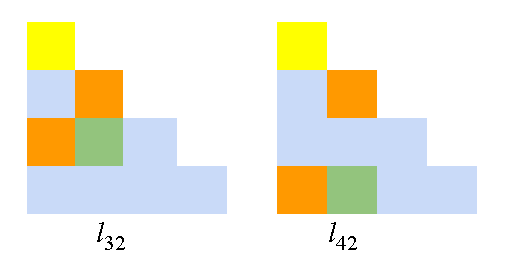
\includegraphics[width=0.5\textwidth]{MatrixGreen}
\end{center}


Los colores en este caso tienen los siguientes distintivos:

\begin{itemize}
\item Verde: El elemento que se esta calculando.
\end{itemize}

\begin{itemize}
\item Naranja: Los elementos de los que depende directamente el elemento calculado.
\end{itemize}

\begin{itemize}
\item Amarillo: Los elementos de los que depende indirectamente el elemento calculado.
\end{itemize}
\end{frame}

\begin{frame}{Algoritmo}{Paso a paso}
El algoritmo para el calculo en paralelo sera:

\begin{enumerate}
\item Se calcula el elemento de la diagonal  $l_{kk}$.
\item Se calculan en paralelo los elementos para cada i con la j fija.
\item Se repite para toda $k <=n$ donde $n$ es la dimension de la matriz, dado que es simetrica tendremos matrices de $nxn$.
\end{enumerate}
\end{frame}

\begin{frame}{Ejemplo grafico}
En el primer punto el calculo depende unicamente de los elementos de la fila $k$, en una matriz de $n=5$ el orden de calculo sera:

\begin{center}
	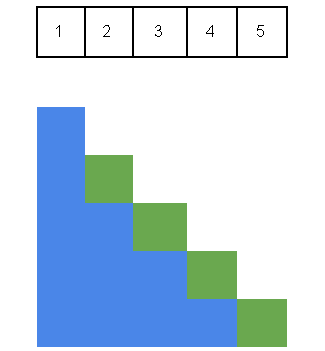
\includegraphics[width=0.25\textwidth]{MatrixBlue}
\end{center}

El orden es de $1 \to 5$ y empezando por el elemento en verde, siendo los elementos en azul ,para cada columna, los que se podran calcular en paralelo.
\end{frame}


\begin{frame}{OpenMP}
\begin{block}{Ventajas de OpenMP}
\begin{itemize}
\item Paralelizar for-loops secuenciales de forma simple
\item Paralelizacion de tareas y sincronizacion explicita de threads
\item Permite una paralelizacion del codigo secuencial de forma paulatina (incremental paralellism)
\end{itemize}
\end{block}
\end{frame}

\begin{frame}{Programacion}
\begin{enumerate}
\item Se diseno y programo en R un script que genera matrices para su posterior implementacion de la Factorizacion Cholesky en C.
	\begin{itemize}
	\item El nombre del archivo que contiene el script es \textbf{matriz.r}.
	\item Se ejecuta con el comando: python \textbf{matriz.r n}, en el cual se debe sustituir \textbf{n} por la dimension de la matriz cuadrada positiva definida a generar.
	\item El resultado se almacenara en el archivo \textbf{matrizSPD.txt} en una sola columna, para despues ser el insumo del algoritmo de factorizacion de cholesky con \textbf{chlesky$\_$final.c}.
	\end{itemize}
\end{enumerate}
\end{frame}

\begin{frame}{Programacion}
\begin{itemize}
\item El script \textbf{cholesky$\_$final.out} realizara mediante standar input la ingesta de los elementos de la matriz y posteriormente imprimir la matriz factor en el archivo: \textbf{fact.txt}. Se dejan los archivos .txt como ejemplo con matrices de dimensión $20 x 20$. 
\item Por ultimo los scripts \textbf{cholesky$\_$1.c} y \textbf{chol$\_$seq.c} son ejemplos de aplicaciones de matrices pequeñas en el algoritmo de la factorizacion cholesky tanto secuencial como en paralelo con tiempos de ejecucion y matrices introducidas a mano en el script.
\end{itemize}
\end{frame}


% Placing a * after \section means it will not show in the
% outline or table of contents.
\section*{Conclusiones}

\begin{frame}{Conclusiones}
  \begin{itemize}
  \item
    The \alert{first main message} of your talk in one or two lines.
  \item
    The \alert{second main message} of your talk in one or two lines.
  \item
    Perhaps a \alert{third message}, but not more than that.
  \end{itemize}
  
  \begin{itemize}
  \item
    Outlook
    \begin{itemize}
    \item
      Something you haven't solved.
    \item
      Something else you haven't solved.
    \end{itemize}
  \end{itemize}
\end{frame}



% All of the following is optional and typically not needed. 
\appendix
\section<presentation>*{\appendixname}
\subsection<presentation>*{Referencias}

\begin{frame}[allowframebreaks]
  \frametitle<presentation>{Referencias}
    
  \begin{thebibliography}{10}
    
  \beamertemplatebookbibitems
  % Start with overview books.

  \bibitem{Author1990}
    A.~Author.
    \newblock {\em Handbook of Everything}.
    \newblock Some Press, 1990.
 
    
  \beamertemplatearticlebibitems
  % Followed by interesting articles. Keep the list short. 

  \bibitem{Someone2000}
    S.~Someone.
    \newblock On this and that.
    \newblock {\em Journal of This and That}, 2(1):50--100,
    2000.
  \end{thebibliography}
\end{frame}

\end{document}